\documentclass[twocolumn,showpacs,preprintnumbers,nofootinbib,prd,
superscriptaddress,10pt]{revtex4-1}

\usepackage{amsmath,amssymb}
\usepackage{amsfonts}
\usepackage[normalem]{ulem}
\usepackage{textcomp}
\usepackage{hyperref}
\usepackage{enumitem}
\usepackage{bm}
\usepackage{afterpage}
\usepackage{graphicx}
\graphicspath{{img/}} %setting img path
\usepackage{psfrag}
\usepackage{mathtools}
\usepackage{tensor}
\usepackage{layouts}
\usepackage{DejaVuSans}
\usepackage{epstopdf}
\usepackage[usenames,dvipsnames]{xcolor}
\usepackage[utf8]{inputenc}
\usepackage{multirow}
\usepackage{algpseudocode}
\usepackage{algorithm}
\usepackage{rotating}
\usepackage{tabularx}
\usepackage{ragged2e}
\usepackage{blindtext}
\usepackage{graphicx}
\usepackage{siunitx}
	\sisetup{output-decimal-marker={.}}
	
	%some math symbols
\newcommand{\R}{\mathbb{R}}
\newcommand{\N}{\mathbb{N}}
\DeclareMathOperator{\sign}{sign}
\renewcommand{\d}[1]{\ensuremath{\operatorname{d}\!{#1}}}
\renewcommand{\dvol}[2]{\ensuremath{\operatorname{d}^{#2}\!{#1}}}
%argmin and argmax
\DeclareMathOperator*{\argmax}{arg\,max}
\DeclareMathOperator*{\argmin}{arg\,min}

\newcommand{\scalar}[2]{\langle #1|#2 \rangle}
\newcommand{\scalarnonorm}[2]{\langle #1|#2 \rangle_{\text{not normalized}}}
\newcommand{\rescalar}[2]{( #1|#2 )}
\newcommand{\imscalar}[2]{[ #1|#2 ]}

% comments command
\newcommand{\stefano}[1]{{\textcolor{blue}{\texttt{SS: #1}} }}
\newcommand{\sarah}[1]{{\textcolor{red}{\texttt{SC: #1}} }}
\newcommand{\oldnewtxt}[2]{\sout{#1}\textcolor{red}{#2}}

\begin{document}

	%%%%%%%%%%%%%%%%%%%%%%%%%%%%%%%%% ABSTRACT
\begin{abstract}
	See paper plan: \href{https://docs.google.com/document/d/1O8z0aDlXtV0LyrtK60vaQDzk9iiCsrjj1ThRGX1tX-0/edit}{google-doc}

\end{abstract}
	
	%%%%%%%%%%%%%%%%%%%%%%%%%%%%%%%%% TITLE
	\title{Metric bank placement}
	\author{Stefano \surname{Schmidt}}
		\email{s.schmidt@uu.nl}
        \affiliation{Nikhef, Science Park 105, 1098 XG, Amsterdam, The Netherlands}
        \affiliation{Institute for Gravitational and Subatomic Physics (GRASP),
Utrecht University, Princetonplein 1, 3584 CC Utrecht, The Netherlands}
        
        %
	\author{Sarah \surname{Caudill}}
		\email{s.e.caudill@uu.nl}
        \affiliation{Nikhef, Science Park 105, 1098 XG, Amsterdam, The Netherlands}
        \affiliation{Institute for Gravitational and Subatomic Physics (GRASP),
Utrecht University, Princetonplein 1, 3584 CC Utrecht, The Netherlands}
	\maketitle

	\tableofcontents

	%%%%%%%%%%%%%%%%%%%%%%%%%%%%%%%%% BODY 
\section{Introduction}

As the gravitational waves astronomy enters in a mature state, the parameter space of Binary Black Holes (BBH) being searched in the interferometer data is constantly increasing. There are already searches targerting the parameter space of sub-solar mass black holes (BH) \cite{}, primordial BHs \cite{} and intermediate mass BHs. Moreover, there is a growing interests in searching for precessing signals and eccentric binaries.
All these efforts requires to generate accurate templates banks that covers the parameter space of interests. This is a highly non trivial and computationally expensive, task and its accuracy is crucial for the outcome of the searches.

The most widely used approach to bank generation ({\it stochastic} method) consists in scattering templates around the parameter space with a rejection technique \sarah{we should cite sbank papers here; think this is the main one: https://arxiv.org/abs/1210.6666}. A proposed template is included in the bank only if its distance between all the other templates is smaller than a given user defined threshold. While this method is very accurate and proved to work in many situation, it is very time consuming. Indeed it requires to generate a huge number of BBH waveforms template and to perform extensive match computations.
As we are moving toward larger banks, that cover more exotic parameter space, such approach may become unfeasibly expensive.

For this reason, there has been a recent growing interest on metric template placing. Such methods rely on approximating the match between two waveforms with a bilinear form. Despite being approximate, this approach allow for a (much) faster template placing that may overcome some of the major limitations of the standard stochastic placement algorithm.
Following the seminal work by Owen \cite{owen_metric}, a large number of approaches that use metric approximation (in some form) have been introduced.

In this work, we develop a novel approach to template placing based on the metric approximation of the match.
Our method is specifically designed for dealing with high-dimensional (more than 4 dimensional) template banks of precessing signals. This makes it particulary suitable for investigating exotic regions for BBH parameter space, enabling generation of banks for precessing and eccentric signals. In such situation, where an established standard bank does not exist, it is crucial to allow for a fast, yet accurate, exploration of different bank configuration.

Our model constructs an internal representation of the paramter space of interests, computes the metric for distance computation and exploits this for fast template placing. \sarah{This is nice. I think you will want to have maybe a diagram that gives an overview of the whole package. For instance, to show how the bank code and injection code can make a workflow that gives you a validated bank.}
The approach is implemented in an open-source python package \texttt{mbank}, freely available on GitHub\footnote{
It available at the repository: \href{https://github.com/stefanoschmidt1995/mbank}{stefanoschmidt1995/mbank}}.
The package offers support for tiling the parameter space of interests and placing templates with an user given average spacing. Moreover, it offers an injection helper that allows for a very fast validation of the bank.
It is designed to run in parallel the most heavy computations.
As a summary, \texttt{mbank} is implemented to be:
\begin{itemize}
	\item Extremely fast \sarah{This will need to be bench-marked. Do you have some timing numbers already?}
	\item Suitable for large banks and high dimensional {\it exotic} parameter space
	\item Fairly accurate
\end{itemize}
\stefano{Shall you explicitly say a common use case??}

The rest of this paper is devoted to present and validate \texttt{mbank}.
In sec.~\ref{sec:methods} we present the details of the bank generation algorithm.
Section~\ref{sec:validation} will be devoted to the validation of the performance of the code. We will focus on the comparison with the widely used stochastic placement code \texttt{sbank}.
To demostrate the capabilities of \texttt{mbank}, we will employ our code to generate two large banks of exotic regions of parameter space: a bank of precessing signals and a bank of eccentric signals. This will be the topic of sec.~\ref{sec:bank_generation}.
Finally, in sec.~\ref{sec:conclusion} we will present some conclusive remarks on our work, with particular attention to future prospects.

	%%%%%%%%%%%%%%%%%%%%%%%%%%%%%%%%%
\section{Methods} \label{sec:methods}

\stefano{This introductory part must be trimmed a lot}
When searching for a BBH signal in the gravitational waves data, it is custom to used a frequentist detection statistics $\Lambda$. It is a measure of the probability ratio between the hypothesis that a signal $s$ is buried in the data and the hypotesis that only noise $n$ is inside th data $d$. In symbols:
\begin{equation}
	\Lambda(\theta) = \log\frac{p(s(\theta)|d)}{p(n|d)}
\end{equation}
where we assume that the signal model is parameterized by a set of parameters $\theta$.
For every given observation time, the search consists in maximizing such probability with respect to $\theta$. 
The generic eccentric BBH signal registered at detector is characterized by 17 quantitities. Luckily, it turns out that one is able to maximize analytically over some of them. For the other quantities, a brute force approach is required: to find the maximum, $\Lambda(\theta)$ is evaluated on a large set of values, usually called {\it template bank}. 

In principle, a template for a generic BBH gravitational waves signal can depend on a set of 12 physical quantities: two BH masses ($m_1$, $m_2$), two 3 dimensional spins $s_1$, $s_2$), the inclination angle $\iota$, the reference phase $\phi$, the eccentricity $e$ of the orbit and the mean periastron anomaly $a$.

Of course, based on some experimental assumptions on the nature of the signal such space can be further reduced to a limited sub-space. Moreover, in some situation is might be possible to maximize analitically the likelihood over certain quantities\footnote{
For example, a common situation is when we look for a non-precessing BBH and we neglect the Higher Order Modes of the waveforms. In this situation, the paramters space to search by brute force has only 4 dimensions (the two masses and the two z components of the spins).}.
In such cases, the parameters that do not enter the bank can be freely neglected (i.e. set to $0$).

It is useful, to think of the BBH parameter space as a D-dimensional manifold $\mathcal{B}_D$ embedded in a large 12 dimensonal manifold $\mathcal{B}$: each point of the manifold corresponds to a GW signal. The number $D$ of dimensions depends on the BBH variables under consideration.

Placing templates on $\mathcal{B}_D$ is a highly non-trivial task, as one has to struggle to ensure a good coverage (to avoid missing any signal) while keeping a low number of templates (to save computational power).
Throughtout the years many different techniques have been devised to achieve such goal.

The general approach consist in equipping $\mathcal{B}_D$ with a distance (called {\it match}) and then placing templates so that they:
\begin{itemize}
	\item cover all the manifold
	\item their mutual distance is as close as possible to a target distance
\end{itemize}
Computing the match (distance) between two templates is a very computationally expensive task, as it requires to generate two templates waveforms for its evaluation. With current waveform generation methods, this operation is very slow and generating a reliable bank can take up to weeks of computation.

This works develops a novel approach to template placing. It is focused on the generation of a high dimensional ($D>4$) banks.
The bank generation (i.e. the placing of templates) is articulated in three logical steps:

\begin{enumerate}
	\item Construction of a metric approximation of the match between templates. This makes $\mathcal{B}_D$ and euclidean manifold.
	\item Creation of a tiling (cover) for the manifold. In each tile the metric is approximately constant.
	\item Placing the templates according to the tiling
\end{enumerate}

Although the template placing is only approximately optimal, this method is order of magnitude faster than the standard approachs, as it avoids to compute a large number of waveforms. For this reason, it allows the creation of large banks on a high dimensional parameter space.
We will devote the rest of this section to go through all the details of the steps above.

\subsection{The metric} \label{sec:metric}

In this section we define a metric distance on the manifold of templates $\mathcal{B}_D$. Such metric approximates the {\it match} between templates and can be used a fast-to-compute surrogate. We will also derive an explicit expression for the metric in terms of the waveform and its gradients.

We can introduce a complex \textit{scalar product}\footnote{
Technically, this is a scalar product on the $L^2$ space of the waveforms $h$ and not (yet) on the D-manifold of the parameters
} between two \textit{waveforms} $h$ as:

\begin{equation} \label{eq:scalar_product}
	\scalar{h(\theta_1)}{h(\theta_2)} = 4 \int_{-\infty}^{\infty} \d{f} \frac{\tilde{h}_+^*(f;\theta_1) \tilde{h}_+(f;\theta_2)}{S_n(f)}
\end{equation}

where $h_+(\cdot; \theta)$ denotes the plus polarization of the waveform evaluated at the point $\theta$ of the manifold, $\tilde{\phantom{h}}$ denotes the Fourier transform and $S_n(f)$ is the power spectral density.
It is important to note that the parameters $\theta$ may not fully specify the BBH parameter space: in this case, the expression $h(\theta)$ assumes that the waveform is generated at some default constant paramters for the quantities not constrained by $\theta$.
We also define $\rescalar{h_1}{h_2} = \Re\scalar{h_1}{h_2}$ and $\imscalar{h_1}{h_2} = \Im\scalar{h_1}{h_2}$.

A waveform $h(\theta)$ can be normalized using the scalar product above:
\begin{equation} \label{eq:normalization}
	\hat{h}(\theta) = \frac{h(\theta)}{\scalar{h(\theta)}{h(\theta)}}.
\end{equation}
If the scalar product is computed between two normalized WFs $\hat{h}$, it will take values between $0$ and $1$.

While eq.~\eqref{eq:scalar_product} can be already used to equip the manifold with a distance, it is more common, due to the details of the statistics used for searches \cite{something}, to introduce a different distance on the manifold.
For each parameter $t$, we define the overlap $\mathcal{O}(\theta_1,\theta_2, t)$ between normalized WFs as:
\begin{align}\label{eq:overlap}
	\mathcal{O}(\theta_1,\theta_2, t) &= \left\| \int\limits_{-\infty}^{+\infty} \d{f} \frac{\tilde{\hat{h}}^*(f;\theta_1)\tilde{\hat{h}}(f;\theta_2) e^{i2\pi ft}}{S_n(f)} \right\| \nonumber\\
	&= \left\| \scalar{\hat{h}(\theta_1)}{\hat{h}(\theta_2)e^{i 2\pi ft}} \right\| 
\end{align}
where, with a slight abuse of notation, we defined $\hat{h}(\theta)e^{i 2\pi ft}$ to be the waveform $\hat{h}(\theta)$ traslated by a constant time $t$.

Based on the overlap, we can eventually define the {\it match} as:
\begin{align}\label{eq:match}
	\mathcal{M}&(\theta_1,\theta_2) = \max_t \mathcal{O}(\theta_1,\theta_2, t) \\
	&= \max_t \sqrt{ \rescalar{\hat{h}(\theta_1)}{\hat{h}(\theta_2)e^{i 2\pi ft}}^2 + \imscalar{\hat{h}(\theta_1)}{\hat{h}(\theta_2)e^{i2\pi ft}}^2 }  \nonumber 
\end{align}

The match definition is motivated by the expression of the detection statistics \cite{something} in use for non-precessing signals. It takes values in the range $[0,1]$ and trivially $\mathcal{M}&(\theta,\theta) = 1$.
It can be used to define a {\it distance}\footnote{
From a strict geometrical point of view, this is not a distance since it does not satisfy triangular inequality. However, this does not affect its effectivness in measuring the ``dissimilarity" between two waveforms, hence two points of the manifold.}
on the D-manifold $\mathcal{B}_D$:
\begin{align}\label{eq:distance}
	d(\theta_1,\theta_2) = \sqrt{1 - \mathcal{M}(\theta_1,\theta_2)}
\end{align}
The distance above is also called {\it mismatch}.

As any smooth function, the mismatch can be approximated by a bilinear form in the neighbourhood of any given point $\theta$. Such bilinear form is represented by a $D\times D$ matrix $M(\theta)$ such that\footnote{
In this expression and everywhere else, we assume Einstein summation convention for vector product.}:
\begin{align}\label{eq:metric_definition}
	d^2(\theta_1,\theta_2) = 1 - \mathcal{M}(\theta_1,\theta_2) \simeq M(\theta)_{ij} \Delta\theta_i \Delta\theta_j
\end{align}
where $\Delta\theta = \theta_1-\theta_2$ is a D-dimensional vector.
The distance induced by the metric approximates the distance between two points of the manifold.

The metric depends on the gradients $\partial_i h(\theta)$ of the waveform and has the following expression:
\begin{equation}\label{eq:metric_expression}
	M(\theta) = - \frac{1}{2} \left( H_{ij} - \frac{H_{ti}H_{tj}}{H_{tt}} \right)
\end{equation}
where $H(\theta)$ is the Hessian of the overlap eq.~\eqref{eq:overlap} (a $D+1$ square matrix). Note that the metric is positive definite.
The details of the computation of the Hessian in terms of the gradients of the waveform are presented in appendix \ref{app:metric}.
The full expression is given in eqs.~\eqref{eq:H_tt_grad}-\eqref{eq:H_ij_grad}.

For most of the waveforms available, the gradients can be evaluated with finite difference methods. For a limited number of Machine Learning based waveform model \cite{something}, such gradients are available analytically (thus speeding up the computation).
The validity and the limitation of eq.~\eqref{eq:metric_definition} will be scrutined in sec.\ref{sec:metric_accuracy}.

Equipped with the metric eq.~\eqref{eq:metric_expression}, the manifold $\mathcal{B}_D$ becomes an Euclidean manifold with line element:
\begin{equation}\label{eq:line_element}
	\d{s^2} = M_{ij}(\theta) \d{\theta_i} \d{\theta_j}
\end{equation}
We can then use standard results from differential geometry to compute distances and volumes. In particular, the volume of a subset $\mathcal{T}$ (tile) of the manifold can be computed as:
\begin{equation}\label{eq:volume_tile}
	\text{Vol}(\mathcal{T}) = \int_\mathcal{T} \dvol{\theta}{D} \; \sqrt{|M(\theta)|}
\end{equation}
where $|\cdot|$ denotes the determinant of a matrix.

It is important to realize that, as any Taylor expansion, this approximation holds only when ${\Delta\theta_i << 1 \; \forall i}$.
\stefano{Keep writing here... Or state this somewhere...}


As a final remark, we note that other definitions for the match are possible (see e.g. \cite{sky_maxed,symphony}). These are motivated by different expressions for the detection statistics, which depends on the assumptions made on the signal (i.e. precessing or eccentric signals or with Higher Order Modes). Here we limit to use the ``vanilla" expression~\eqref{eq:match} for aligned spins BBH (for which $\tilde{h}_+ \propto i \tilde{h}_\times$), even for cases where it does not hold. We expect the error introduced by this to be negligible.

\subsection{The tiling} \label{sec:tiling}

In principle the metric is a continuos quantity, defined at every point of the space. However, as the computation of the metric is expensive it is unfeasible to compute the metric at every point of the space.
For this reason, the parameter space of interests (geometrically the manifold $\mathcal{B}_D$) should be divided into different {\it tiles} (subset). The assumption is that, in each tile, the metric can be approximated as a constant.
The validity of this assumption will be assesed in sec.~\ref{sec:tiling_accuracy}.

To simplify the geometry (and make the computation faster), we only consider hyper-cubes as tiles. A tile $\mathcal{T}$ is then an ordered couple:
\begin{equation} \label{eq:tile}
	\mathcal{T} = \left(R_{[\theta_{min}, \theta_{max}]}, M \right)
\end{equation}
where $R_{[\theta_{min}, \theta_{max}]}$ is an hyper-cube (rectangle) with extrema $\theta_{min/max}$ and where $M$ is the metric evaluated at the center of the tile $\frac{\theta_{min}+\theta_{max}}{2}$.

To tile the space we use the iterative algorithm described in alg.~\ref{alg:tiling}.
Given an initial tile, that covers the whole space of interests, the algorithm returns a list of tiles, covering the original space.
The number of tiles is controlled by a parameter $V_{tile}$ which is an indirect measure of the (metric) volume. It is defined as:
\begin{equation} \label{eq:templates}
	V_{tile} = \frac{Vol(R_{[\theta_{min}, \theta_{max}]}) \sqrt{|M|}}{0.1^D}
\end{equation}
where $0.1$ is a reference distance.
$V_{tile}$ has a straightforward interpretation: under certain assumptions (see sec.~\ref{sec:template_placing}), it is the number of templates that should lie into the tile if their spacing is exactly $0.1$.
The choice of this parameter makes sure that all the tiles cover approximately the same volume, thus keeping the same number of templates: the smaller $V_{tile}$ the more accurate is the coverage of the space (hence the higher is the computational cost).

As we limit to rectangular tiles, \texttt{mbank} is not able to deal with a non rectangular boundaries for the parameter space. This is of course a strict limitation, as the typical user may want to impose non cubic boundaries. However, due to the speed of the bank generation, a feasible approach to overcome such restriction is to generate the bank on a large domain of interest and imposing any non-linear boundary as a post processing step. \stefano{shall we implement this??? Given the new random approach it shouldn't be too difficult...}

\begin{algorithm}[t!]
\caption{Tiling}
\begin{algorithmic}
	\State WRITEME
	\State $i \gets 10$
	\If{$i\geq 5$} 
		\State $i \gets i-1$
	\Else
		\If{$i\leq 3$}
		    \State $i \gets i+2$
		\EndIf
	\EndIf
\end{algorithmic}
\label{alg:tiling}
\end{algorithm}

\subsection{Template placing} \label{sec:template_placing}

Once a tiling is available, we need to place the templates that will be part of the bank.
As it is common, the input parameter controlling the number of templates (and their spacing) is the so-called {\it minimum match} $MM$. It is defined as the minimum tolerable match that a random injection (inside the relevant space) must have with the templates of the bank.
The optimal template arrangment should be on a grid with constant spacing $d(MM)$. While for some methods arranging templates on a grid may be hard, the grid spacing $d(MM)$ still makes sense as an {\it average} spacing.

Following an argument by Owen \cite{owen_metric}, the optimal distance between templates should be:
\begin{equation}
	d(MM) = 2 \sqrt{\frac{1-MM}{D}}
\end{equation}
This will be the input to any template placing method.

Several templates methods have been implemented, each of which has their strength. The available placing methods (and their pros and cons) are listed in Table~\ref{tab:placing_methods}.

Below we describe briefly each of them. The recommended one is ...

\paragraph{Random}\label{par:random}
\paragraph{Geometric}\label{par:geometric}
\stefano{Do we want to do an appendix for the geometric placement? \ref{app:placing}}
\paragraph{Stochastic}\label{par:stochastic}
\paragraph{Geo-Stochastic}\label{par:geostochastic}
\paragraph{Tile-Stochastic}\label{par:tilestochastic}
\paragraph{Uniform}\label{par:uniform}
\stefano{Where do we want to say that Owen law is very limited in scope??}
\paragraph{Iterative}\label{par:iterative}


\begin{table}[t!]
	\centering
	 \begin{tabular}{l c c c} 
	 \hline
	 \phantom{Method} & Single Tile & Multiple Tiles & Speed \\
	 \hline
	 Random & 6 & 87837 & 787 \\ 
	 Geometric & 7 & 78 & 5415 \\
	 Stochastic & 545 & 778 & 7507 \\
	 Geo-Stochastic & 545 & 18744 & 7560 \\
	 Tile-Stochastic & 88 & 788 & 6344 \\ 
	 Uniform & 88 & 788 & 6344 \\ 
	 Iterative & 88 & 788 & 6344 \\ 
	 \hline
	 \end{tabular}
	 \caption{A schematic comparison of the different placing methods implemented \stefano{We need to think about this...}}
 	 \label{tab:placing_methods}
\end{table}

	%%%%%%%%%%%%%%%%%%%%%%%%%%%%%%%%%
\section{Validation} \label{sec:validation}

\sarah{Here we will want a few different types of tests and plots:\\
* You will want some plots showing what the template banks look like\\
* Might also be nice to zoom in on a cell or demonstrate some of the details of the bank placement with a plot or two\\
* You will want to describe the injection set used to test the coverage of each bank you make (could use a table for this)\\
* You will want a plot showing the recovery of these injections as a function of their parameter space (see for example Fig 7-11 here: https://arxiv.org/pdf/1812.05121.pdf)\\
* You will want a plot showing the speed of your code compared to a conventional method (the benchmarking I mentioned earlier) \\
* 
 }

\subsection{Metric accuracy} \label{sec:metric_accuracy}

\begin{figure}[h]
	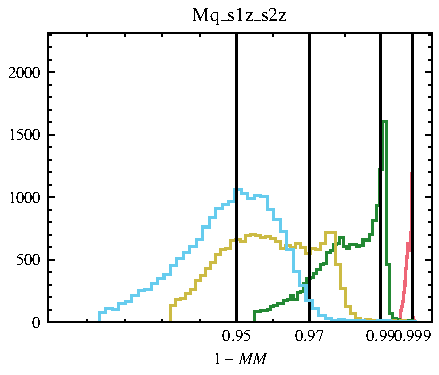
\includegraphics{metric_accuracy_Mq_s1z_s2z}
	\caption{Metric accuracy, for different variable formats \sarah{what are the different colors here?}}
	\label{fig:metric_accuracy}
\end{figure}

Histogram with the actual match for points with a constant metric match

\subsection{Tiling accuracy} \label{sec:tiling_accuracy}

\begin{figure}[h]
	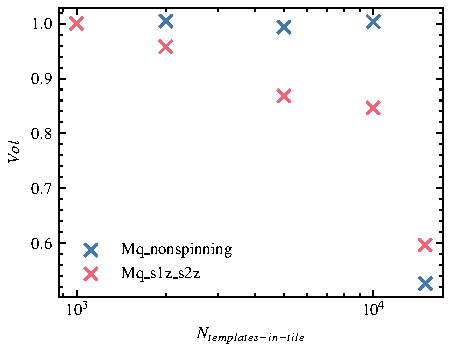
\includegraphics{tiling_accuracy_test}
	\caption{Tiling accuracy}
	\label{fig:tiling_accuracy}
\end{figure}

Compute the match computed with the tiling vs the actual match.

\subsection{Comparison with \texttt{sbank} }

\begin{figure}[h]
	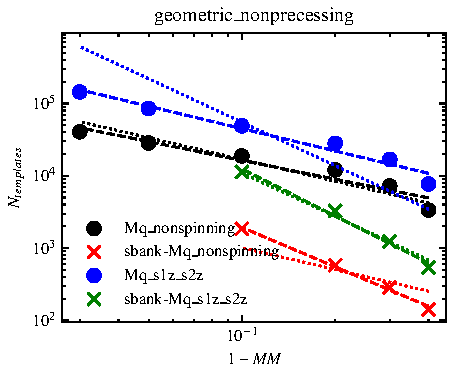
\includegraphics{bank_scaling_nonprecessing_geometric}
	\caption{Scaling for the bank, compared with sbank}
	\label{fig:bank_scaling}
\end{figure}

Generating 2/3 small non-precessing banks with both \texttt{mbank} and \texttt{sbank}.
Comparison based on:
	\begin{itemize}
		\item size
		\item effectualness
		\item speed
	\end{itemize}

Include scaling plots.

	%%%%%%%%%%%%%%%%%%%%%%%%%%%%%%%%%
\section{Bank generation: two case studies} \label{sec:bank_generation}

Useful to present the features of these two banks generated?

\subsection{A precessing bank}
This could be the bank we use for precessing searches.

\subsection{An eccentric bank}
This could be a nonspinning, eccentric bank. It should have 500K templates for a reasonable range of masses.

\section{Final remarks and future prospects} \label{sec:conclusion}
Usual stuff

	%%%%%%%%%%%%%%%%%%%%%%%%%%%%%%%%% ACKNOWLEDGMENTS
        \begin{acknowledgments}
         
          WRITEME...
        \end{acknowledgments}

	%%%%%%%%%%%%%%%%%%%%%%%%%%%%%%%%% APPENDIX
\appendix
\section{Details of the metric computation}\label{app:metric}

In this appendix we report the details of the derivation of the expression~\eqref{eq:metric_expression}, as well as the computation of the Hessian $H$ of the overlap eq.~\eqref{eq:overlap} in terms of the gradients of the waveform $h(\theta)$. 

We begin by expanding the quantity $\mathcal{M}(\theta,\theta +\Delta\theta)$ for $\Delta\theta$ around $0$. Since the $\mathcal{M}(\theta,\theta +\Delta\theta)$ has a maximum for $\Delta\theta = 0$, the leading term is quadratic in $\Delta\theta$.
We obtain:
\begin{align} \label{eq:metric_derivation}
	&\mathcal{M}(\theta,\theta +\Delta\theta) = \max_{\Delta t} \mathcal{O}(\theta, \theta + \Delta\theta, \Delta t) \nonumber\\
	& =	\max_{\Delta t} \left\{ 1+ \frac{1}{2}\left[ \partial_{ij}\mathcal{O} \Delta\theta_i \Delta\theta_j + 2  \partial_{it}\mathcal{O} \Delta\theta_i \Delta t + \partial_{tt}\mathcal{O} (\Delta t)^2 \right] \right\}  \nonumber \\
	&= 1 + \frac{1}{2}\left[ \partial_{ij}\mathcal{O} - \frac{\partial_{it}\mathcal{O} \partial_{jt}\mathcal{O}}{\partial_{tt}\mathcal{O}}\right] \Delta\theta_i \Delta\theta_j
\end{align}
where all the derivatives are evaluated at ${\Delta\theta = \Delta t = 0}$ and the explicit time maximization yields
${\Delta t = -\frac{\partial_{it}\mathcal{O} \Delta\theta_i}{\partial_{tt}\mathcal{O}}}$.

From the above eq.~\eqref{eq:metric_derivation}, we can read the expression for the metric in eq.~\eqref{eq:metric_expression} recognizing in the derivatives $\partial\partial\mathcal{O}|_{\Delta\theta, \Delta t = 0}$ the components of the Hessian matrix $H$ of the overlap.

We now compute the Hessian of the overlap as a function of the gradients of the {\it normalized} waveforms.
We have\footnote{
A constant factor in front of the frequency in the fourier transform does not affect the result. For this reason, we dropped the constant $2\pi$ in the exponential.}:
\begin{align}
	\partial_i \mathcal{O} &= \frac{1}{\mathcal{O}} \left[ \rescalar{\hat{h}}{\hat{h}e^{ift}}\rescalar{\hat{h}}{\partial_i\hat{h}e^{ift}} + \imscalar{\hat{h}}{\hat{h}e^{ift}}\imscalar{\hat{h}}{\partial_i\hat{h}e^{ift}} \right]\\
	\partial_t \mathcal{O} &= \frac{1}{\mathcal{O}} \left[ \rescalar{\hat{h}}{\hat{h}e^{ift}}\rescalar{\hat{h}}{\hat{h}if e^{ift}} + \imscalar{\hat{h}}{\hat{h}e^{ift}}\imscalar{\hat{h}}{\hat{h}if e^{ift}} \right]
\end{align}
Differentiating another time, after some rearrengments, we get:
\begin{align}
H_{tt} &= \frac{\partial^2 \mathcal{O}}{\partial t \partial t } \left|_{\Delta\theta, t = 0}
								= \rescalar{\hat{h}}{\hat{h}f}^2 - \rescalar{\hat{h}}{\hat{h}f^2} \label{eq:H_tt}\\
H_{ti} &= \frac{\partial^2 \mathcal{O}}{\partial \Delta \theta_i \partial t } \left|_{\Delta\theta, t = 0}
								= - \imscalar{\hat{h}}{\partial_i \hat{h}f} + \imscalar{\hat{h}}{\partial_i\hat{h}} \rescalar{\hat{h}}{\hat{h}f} \label{eq:H_ti}\\
H_{ij} &= \frac{\partial^2 \mathcal{O}}{\partial \Delta \theta_i \partial \Delta \theta_j }\left|_{\Delta\theta, t = 0}
								= \rescalar{\hat{h}}{\partial_i\partial_j\hat{h}} +\imscalar{\hat{h}}{\partial_i\hat{h}} \imscalar{\hat{h}}{\partial_j\hat{h}} \label{eq:H_ij}
\end{align}

To move further, we express the normalized waveform derivatives in terms of the non normalized ones. We get:
\begin{align*}
	\bullet&\quad \partial_i \scalar{h}{h} = \scalar{\partial_i h}{h}+ \scalar{h}{\partial_i h} = 2 \rescalar{h}{\partial_i h} \\
	\bullet&\quad \partial_i \hat{h} =\frac{1}{\rescalar{h}{h}^{3/2}} \left[ \rescalar{h}{h}\partial_i h -  \rescalar{h}{\partial_i h} h \right]	\\
	\bullet &\quad \partial_i \partial_j \hat{h} = \frac{1}{\rescalar{h}{h}^{1/2}} \partial_{ij}h 	+3 \frac{1}{\rescalar{h}{h}^{5/2}} \rescalar{h}{\partial_i h}\rescalar{h}{\partial_j h}h \\
	&- \frac{1}{\rescalar{h}{h}^{3/2}} \left[\rescalar{h}{ \partial_{ij} h} h + \rescalar{\partial_i h}{\partial_j h}  h
		+2\rescalar{h}{\partial_{(i} h} \partial_{j)} h \right]
\end{align*}
where $A_{(ij)} = \frac{1}{2}(A_{ij}+A_{ji})$ denotes symmetrization.

Plugging this into the equations~\eqref{eq:H_tt}-\eqref{eq:H_ij}, we get:
\begin{align}
	H_{tt} &= \frac{1}{\rescalar{h}{h}^{2}} \rescalar{{h}}{{h}f}^2 - \frac{1}{\rescalar{h}{h}} \imscalar{h}{{h} f^2 } \label{eq:H_tt_grad} \\
	H_{ti} &= \frac{1}{\rescalar{h}{h}^{2}} \Big\{ \imscalar{h}{\partial_i {h}} \rescalar{{h}}{{h}f} +\rescalar{h}{\partial_i {h}} \imscalar{h}{hf} \Big\} \nonumber \\
	&- \frac{1}{\rescalar{h}{h}} \imscalar{h}{\partial_i{h} f } \label{eq:H_ti_grad} \\
	H_{ij} &=  \frac{1}{\rescalar{h}{h}^{2}} \Big\{ \rescalar{h}{\partial_i {h}} \rescalar{{h}}{\partial_j {h}} +\imscalar{h}{\partial_i {h}} \imscalar{h}{\partial_j {h}} \Big\} \nonumber \\
	&- \frac{1}{\rescalar{h}{h}} \rescalar{\partial_i h}{\partial_j {h}} \label{eq:H_ij_grad} 
\end{align}

Such expressions, togheter with eq.~\eqref{eq:metric_expression} fully specify the metric computation.
The gradients $\partial_i h$ of the waveform can be computed with an accurate finite difference scheme.



\section{Details of the geometric template placing}\label{app:placing}

\blindtext
\blindtext
	%%%%%%%%%%%%%%%%%%%%%%%%%%%%%%%%% BIBLIOGRAPHY
	\bibliography{biblio.bib}
	\bibliographystyle{ieeetr}

\end{document}



